\documentclass{article}

\usepackage{graphicx}
\usepackage{float}
\usepackage{amsmath}

%The following package imports and styling was obtained from: https://tex.stackexchange.com/questions/348651/c-code-to-add-in-the-document
\usepackage{xcolor}
\usepackage{listings}

\definecolor{mGreen}{rgb}{0,0.6,0}
\definecolor{mGray}{rgb}{0.5,0.5,0.5}
\definecolor{mPurple}{rgb}{0.58,0,0.82}
\definecolor{backgroundColour}{rgb}{0.95,0.95,0.92}

\usepackage[colorlinks]{hyperref}
\hypersetup{citecolor=DeepPink4}
\hypersetup{linkcolor=DarkRed}
\hypersetup{urlcolor=blue}
\usepackage{cleveref}

\lstdefinestyle{CStyle}{
    backgroundcolor=\color{backgroundColour},   
    commentstyle=\color{mGreen},
    keywordstyle=\color{magenta},
    numberstyle=\tiny\color{mGray},
    stringstyle=\color{mPurple},
    basicstyle=\footnotesize,
    breakatwhitespace=false,         
    breaklines=true,                 
    captionpos=b,                    
    keepspaces=true,                 
    numbers=left,                    
    numbersep=5pt,                  
    showspaces=false,                
    showstringspaces=false,
    showtabs=false,                  
    tabsize=2,
    language=C
}

\begin{document}
\title{Sfwr Eng 4F03: Final Project}

\author{Kelvin Lin\hspace{10mm}MacID:linkk4\hspace{10mm}Student Number: *********\\Prabhbir Pooni\hspace{10mm}MacID: poonip\hspace{10mm}Student Number: *********\\Yanting Zhang\hspace{10mm}MacID: zhang169\hspace{10mm}Student Number: *********}

\maketitle

\section{Question 1}
Using \texttt{MPIHost}, timing, speed-up, and efficiency plots were generated for 1, 2, 4, 8, 16, and 32 processors. The program was tested with 2000, 4000, 8000, 16000, and 32000 particles. 9 major steps were used with 1 substep in between. The image produced was 2550 pixels in width by 1960 pixels in height.

For each section, two graphs will be presented. The first graph shows metrics for a pure MPI implementation, while the second graph shows metrics for an MPI implementation optimized with OpenMP.

\subsection{Timing Plot}
The following graphs are timing plots for the different image sizes, different number of particles, and different number of processors. Each line represents a different number of particles. The x-axis represents the number of processors while the y-axis represents the time it took to run the program.

\subsubsection{Pure MPI}
\begin{figure}[H]
	\begin{center}
		\hspace*{-0.5cm}                                                           
  		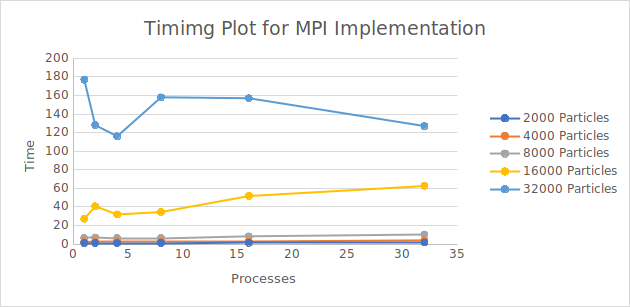
\includegraphics[scale=0.83]{Report_Assets/timingmpi.png}
  	\end{center}
  	\caption{The timing plot with varying the number of processors and particles in MPI}
\end{figure}

\subsubsection{MPI Optimized with OpenMP}
\begin{figure}[H]
	\begin{center}
		\hspace*{-0.5cm}                                                           
  		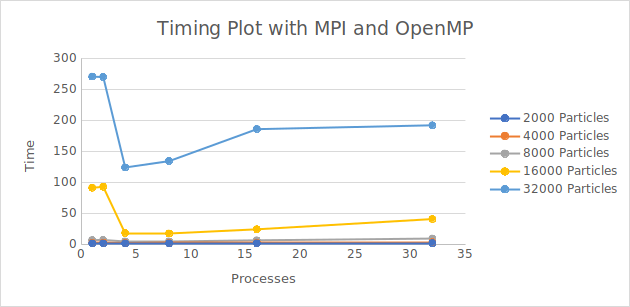
\includegraphics[scale=0.83]{Report_Assets/timingomp.png}
  	\end{center}
  	\caption{The timing plot with varying the number of processors and particles in MPI with OpenMP}
\end{figure}

\subsection{Speedup Plot}
The following graphs are speedup plots for the different image sizes, different number of particles, and different number of processors.

Each line represents a different number of particles. The x-axis represents the number of processors used, while the y-axis represents the speedup observed.

\subsubsection{Pure MPI}
\begin{figure}[H]
	\begin{center}
		\hspace*{-0.5cm}                                                           
  		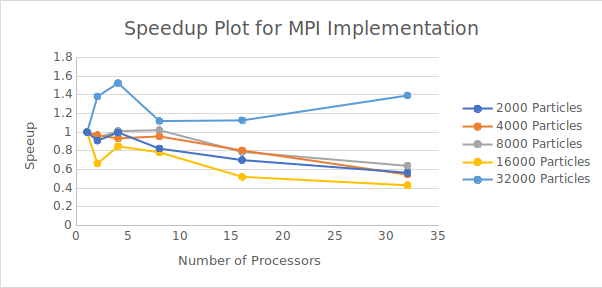
\includegraphics[scale=0.71]{Report_Assets/speedupmpi.png}
  	\end{center}
  	\caption{The speedup plot with varying the number of processors and particles in MPI}
\end{figure}

\subsubsection{MPI Optimized with OpenMP}
\begin{figure}[H]
	\begin{center}
		\hspace*{-0.5cm}                                                           
  		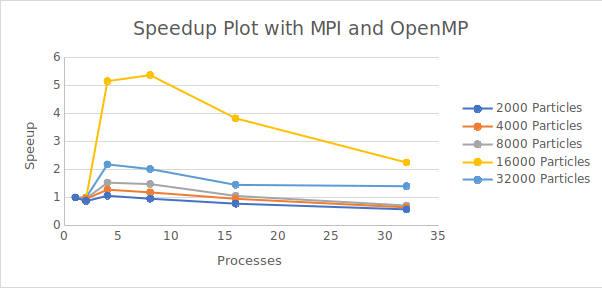
\includegraphics[scale=0.71]{Report_Assets/speedupomp.png}
  	\end{center}
  	\caption{The speedup plot with varying the number of processors and particles in MPI with OpenMP}
\end{figure}

\newpage
\subsection{Efficiency Plot}
The following graphs are efficiency plots for the different image sizes, different number of particles, and different number of processors.

Each line represents a different number of particles. The x-axis represent the different number of processors used, while the y-axis represents the efficiency.

\subsubsection{Pure MPI}
\begin{figure}[H]
	\begin{center}
		\hspace*{-0.5cm}                                                           
  		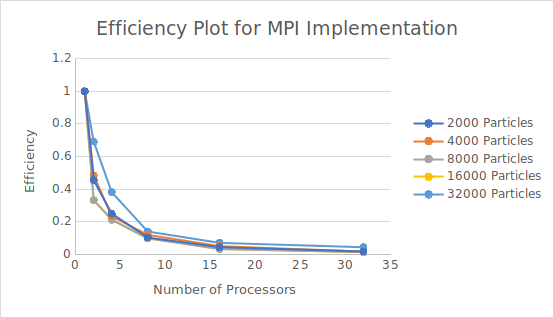
\includegraphics[scale=0.65]{Report_Assets/efficiencympi.png}
  	\end{center}
  	\caption{The efficiency plot with varying the number of processors and particles in MPI}
\end{figure}

\subsubsection{MPI Optimized with OpenMP}
\begin{figure}[H]
	\begin{center}
		\hspace*{-0.5cm}                                                           
  		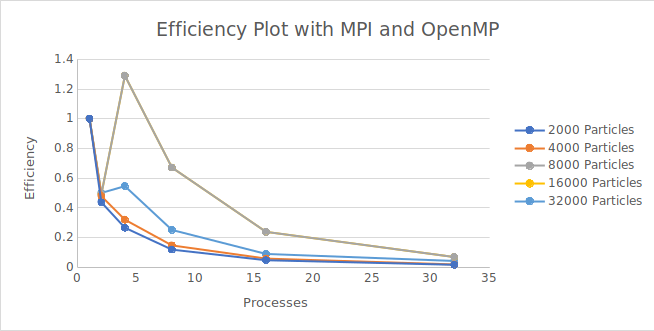
\includegraphics[scale=0.6]{Report_Assets/efficiencyomp.png}
  	\end{center}
  	\caption{The efficiency plot with varying the number of processors and particles in MPI with OpenMP}
\end{figure}

\section{Question 2}
The algorithms are neither strongly nor weakly scalable.

\subsection{Strong Scalability}
A strongly scalable algorithm is an algorithm where given a fixed problem size, as the number of processors increase, the efficiency stays about the same.

If an algorithm is strongly scalable, then an approximately straight horizontal line should be observed in Figure 5. Figure 5 shows whether an algorithm is strongly scalable because each line shows the efficiency of the processors for a fixed problem size as the number of processors used increases.

From Figure 5, it is clear that the efficiency decreases in an exponential fashion for all input sizes. Accordingly, the algorithm is not strongly scalable.

Similar analysis was done with the tuned program using Figure 6. From Figure 6, it is also clear that the efficiency decreases in an exponential fashion for all input sizes. Accordingly, the algorithm is also not strongly scalable.

\subsection{Weak Scalability}
A weakly scalable algorithm is an algorithm where, as the problem size and the number of processors scale at the same rate, the efficiency stays about the same.

To determine weak scalability, a plot mapping the efficiency as the number of processors and the problem size scales uniformly was created. In the plots below, the x-axis represents the number of processors while the y-axis represents the efficiency. The problem size as a tuple of \texttt{(number of processors, problem size)} is {(1, 2000), (2, 4000), (4, 8000), (8, 16000), (16, 32000)}.

\begin{figure}[H]
	\begin{center}
		\hspace*{-0.5cm}                                                           
  		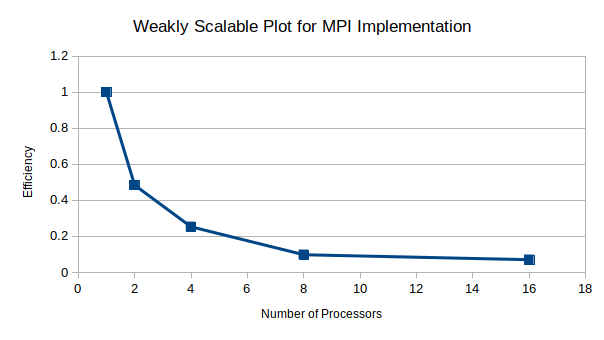
\includegraphics[scale=0.7]{Report_Assets/weakscalempi.png}
  	\end{center}
  	\caption{A plot showing whether the pure MPI version is weakly scalable}
\end{figure}

\begin{figure}[H]
	\begin{center}
		\hspace*{-0.5cm}                                                           
  		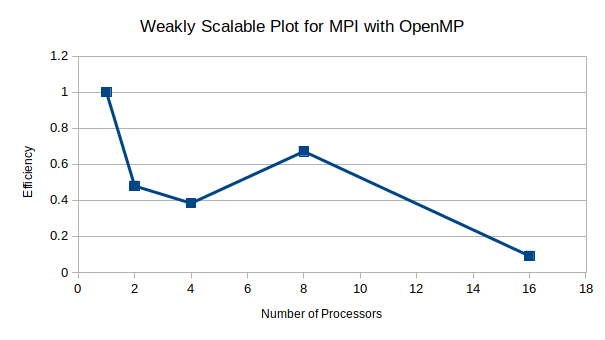
\includegraphics[scale=0.8]{Report_Assets/weakscaleomp.png}
  	\end{center}
  	\caption{A plot showing whether the MPI optimized with OpenMP version is weakly scalable}
\end{figure}

If the algorithm was weakly scalable, then an approximately straight line should be observed in Figures 7 and 8. 

From Figure 7, it is clear that the efficiency decreases exponentially as the number of processors and the problem size linearly increases for the pure MPI implementation. Accordingly, the pure MPI version is not weakly scalable.

From Figure 8, it is clear that the efficiency decreases as the number of processors and the problem size linearly increases for the MPI optimized with OpenMP version. Accordingly, the MPI optimized with OpenMP implementation is not weakly scalable.

\newpage
\section{Question 3}
\subsection{Pure MPI}
\subsubsection{Timing}
In Figure 1, for 32000 particles, the time it takes decreases from 1 processor to 4 processors; however, the time then increases at 8 processors and then slowly decrease. The reason for this decrease may be because the arrangement of data is might have been better aligned when there were 2 or 4 processors opposed to when there were more. The increase in overhead of data transfer may have offset the benefits of additional processors, which is why the time increased after 4 processors.

Similarly, for 16000 particles, the time taken increased from 1 processor to 2 processors, decreased from 2 processors to 4 processors, and then slowly increased thereafter. The timing observed may be due to the same reason mentioned above. The time taken to split data between 2 processors might have significantly offset the computation time. 4 processors minimized the amount of data transfer which allowed for the minimum processing time. Thereafter, the computational power grew at a slower rate than the data transfer time, which caused the timing to slowly increase.

There were no anomalies from 2000 to 4000 particles, perhaps because the input size was not big enough to be a computational challenge for the CPU.

\subsubsection{Speedup}
In Figure 2, for both 16000 and 32000 particles, the speedup increased from 1 to 4 processors, but then decreased from 8 to 16 processors. This reflects the patterns observed in Figure 1. Since the data was better aligned with 1, 2, and 4 processors, there was a greater speedup, but afterwards, the cost of data transfer outweighed the benefits of additional computation power, which caused the slowdown to decrease.

There were no anomalies from 2000 to 4000 particles, perhaps because the input size was not big enough to be a computational challenge for the CPU.

\subsubsection{Efficiency}
In Figure 3, the efficiency for both 16000 and 32000 decreased slower from 1 processor to 4 processors than the others because of the data alignment issue outlined in the previous two sections. 

There were no anomalies from 2000 to 4000 particles, perhaps because the input size was not big enough to be a computational challenge for the CPU.


\end{document}
